%%%%%%%%%%%%%%%%%%%%%%%%%%%%%%%%%%%%%%%%%%%%
% https://github.com/martinhelso/uioposter %
%%%%%%%%%%%%%%%%%%%%%%%%%%%%%%%%%%%%%%%%%%%%
% Class options                            %
%%%%%%%%%%%%%%%%%%%%%%%%%%%%%%%%%%%%%%%%%%%%
% Orientation:                             %
% portrait (default), landscape            %
%                                          %
% Paper size:                              %
% a0paper (default), a1paper, a2paper,     %
% a3paper, a4paper, a5paper, a6paper       %
%                                          %
% Language:                                %
% english (default), norsk                 %
%%%%%%%%%%%%%%%%%%%%%%%%%%%%%%%%%%%%%%%%%%%%
\documentclass[a0paper]{uioposter}


\usepackage{lipsum}                                % Dummy text
\usepackage[figwidth = 0.98\linewidth]{todonotes}  % Dummy image (and more!)
\usepackage[absolute, overlay]{textpos}            % Figure placement
\usepackage{polyglossia}
\usepackage{graphicx}
\usepackage{subcaption}
\setmainlanguage{czech}
\setotherlanguages{english}
\usepackage[mono=true]{libertinus-otf}
\usepackage{microtype}
\setlength{\TPHorizModule}{\paperwidth}
\setlength{\TPVertModule}{\paperheight}


\title{Konceptuální modelování pomocí schematických kategorií}
\author {Dennis Pražák}
%% Optional:
%\institute
%{
%    \inst{1} Department of Mathematics
%    \and
%    \inst{2} Department of Informatics
%}
% Or:
%\institute{Contact information}


%% Remove footline:
%\setbeamertemplate{footline}{}


\begin{document}
\begin{frame}
  \begin{columns}[onlytextwidth]


    \begin{column}{0.5\textwidth - 1.5cm}
      \begin{block}{Úvod}
        Konceptuální modely jako ER a UML byly vyvinuty v době, kdy měl největší zastoupení v databázových systémech jeden logický model -- relační.
        V dnešní době se však kromě relačního modelu ve vyšší míře používá mnoho odlišných logických modelů (grafový, dokumentový, key-value, wide column\dots).

        \alert{Schematické kategorie} jsou nový prostředek ke konceptuálnímu modelování, který je obecnější (má vyšší vyjadřovací schopnost) a není natolik provázaný s logickou vrstvou.
        Schematické kategorie splňují vlastnosti teorie kategorií a lze na ně tak aplikovat již vybudované nástroje tohoto oboru matematiky.

        Cílem této práce bylo vytvořit webovou aplikaci, která umožní konceptuální modelování pomocí schematických kategorií v již známém modelu Entity-Relationship.
        ER schéma se automaticky převede na schematické kategorie.
        Usnadní tak výzkumníkům a potenciálním uživatelům schematických kategorií prozkoumání a seznámení se s tímto novým konceptem.
      \end{block}

      \begin{block}{Příklad diagramů}
        \begin{figure}
          \centering
          \begin{subfigure}{0.45\textwidth}
            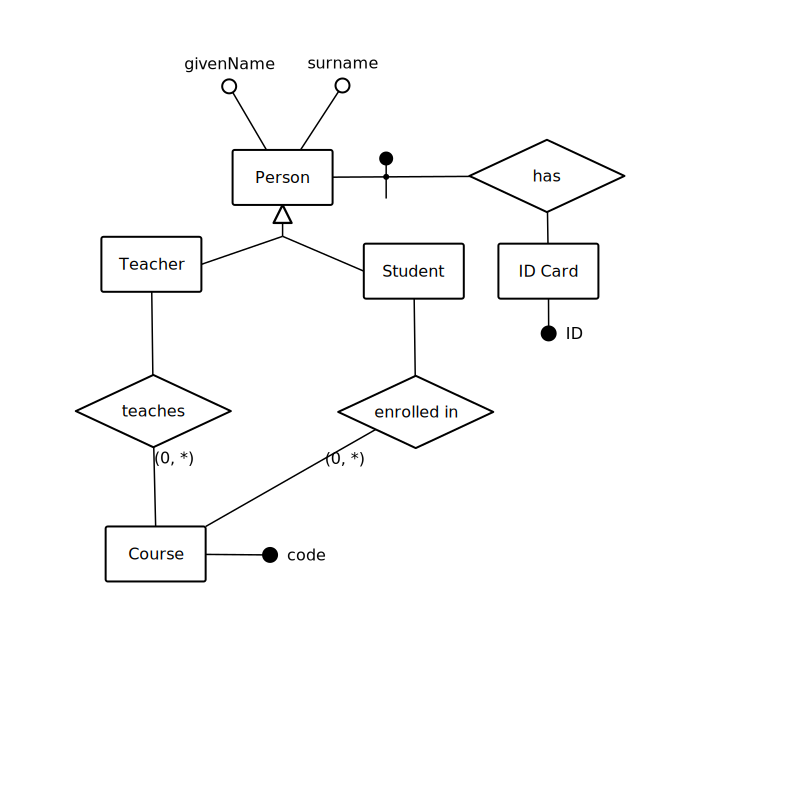
\includegraphics[width=1\textwidth]{./images/university-er.pdf}
            \caption{Entity-Relationship}
          \end{subfigure}
          \begin{subfigure}{0.45\textwidth}
            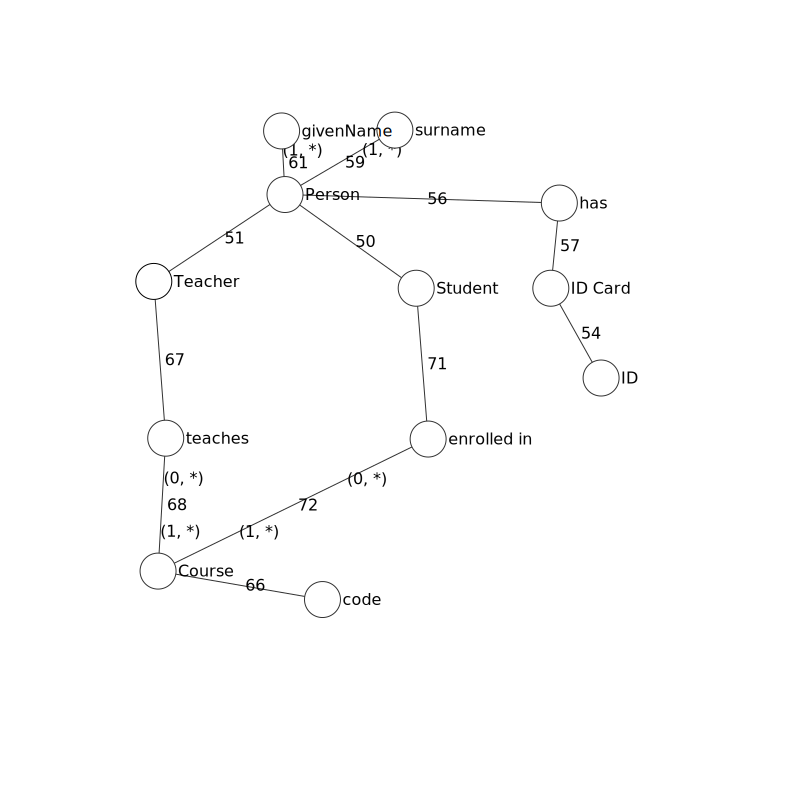
\includegraphics[width=\textwidth]{./images/university-schemcat.pdf}
            \caption{Schematická kategorie}
          \end{subfigure}
          \begin{subfigure}{0.45\textwidth}
            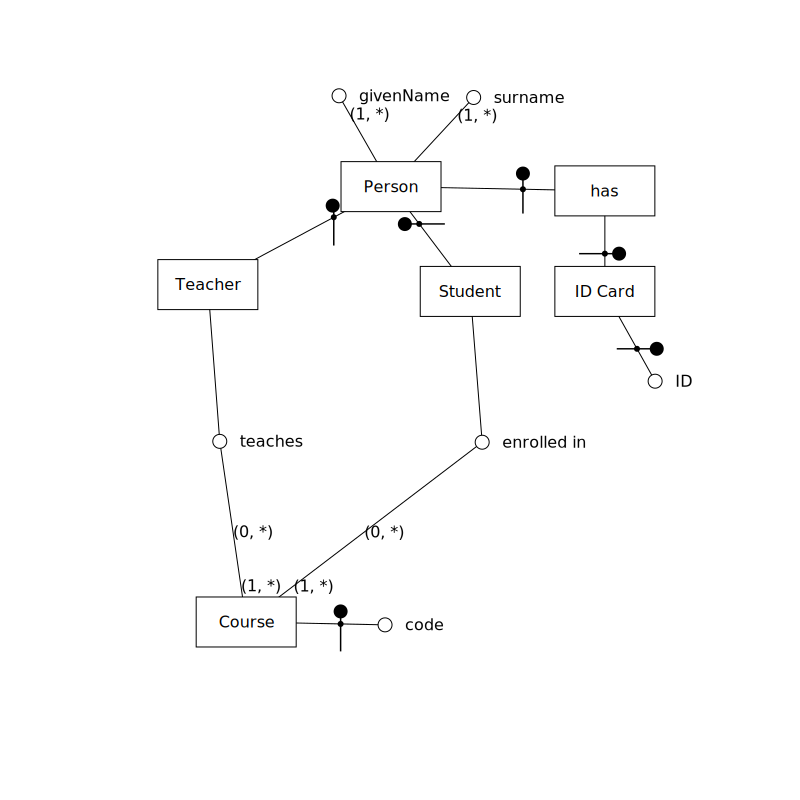
\includegraphics[width=\textwidth]{./images/university-scv.pdf}
            \caption{Vizualizace schematické kategorie}
          \end{subfigure}
        \end{figure}
      \end{block}
    \end{column}


    \begin{column}{0.5\textwidth - 1.5cm}
      \begin{block}{Uživatelské rozhraní}
        \begin{figure}
          \centering
          \includegraphics[width=0.8\textwidth]{./images/identifier-screenshot.png}
        \end{figure}
      \end{block}
      \begin{block}{Závěr}
          Webová aplikace je 
      \end{block}
    \end{column}
  \end{columns}


  \begin{textblock}{0.5}(0.63, 0.935)
    \color{white}
    \sffamily
    \begin{tabular}{rl}
      Vedoucí:    & RNDr.~Martin Svoboda,~PhD.
      \\
      Pracoviště: & Katedra softwarového inženýrství
    \end{tabular}
  \end{textblock}


\end{frame}
\end{document}
